% Problems, Chapter 9: Partial Differential Equations
% Arfken, Weber & Harris, Mathematical Methods for Physicists, 7th ed.
% Requires: amsmath, amssymb, tikz

\section*{Problems}

\Needspace{9\baselineskip}
\subsection*{9.2 First-Order Equations}

Find the general solutions of the PDEs in Exercises 9.2.1 to 9.2.4.

\Needspace{5\baselineskip}
\par\bigskip
\noindent\textbf{9.2.1}\quad
$\dfrac{\partial\psi}{\partial x}+2\dfrac{\partial\psi}{\partial y}+(2x-y)\psi=0$.
\solution
Let $s=x$ and $u=y-2x$, so $y=u+2s$.  The chain rule gives
\[
\partial_x=\partial_s-2\partial_u,\qquad
\partial_y=\partial_u,\qquad 2x-y=2s-(u+2s)=-u.
\]
Hence $\partial_x+2\partial_y=\partial_s-2\partial_u+2\partial_u=\partial_s$,
and the PDE reduces, at fixed $u$, to
$\psi_s-u\psi=0$.  Multiplying by $e^{-us}$ gives
$\partial_s(e^{-us}\psi)=e^{-us}(\psi_s-u\psi)=0$, so
$e^{-us}\psi=F(u)$ does not depend on $s$.  Returning to $s=x$,
$u=y-2x$,
\[
\boxed{\psi(x,y)=e^{x(y-2x)}F(y-2x)},
\]
where $F$ is an arbitrary differentiable function; this includes the zero
solution and does not require taking $\ln\psi$.
Indeed $D=\partial_x+2\partial_y$ annihilates $u$ and satisfies
$D(xu)=u$, hence $D\psi=u\psi=-(2x-y)\psi$.
The coordinate map has determinant one, so it loses no local solutions.


\Needspace{5\baselineskip}
\par\bigskip
\noindent\textbf{9.2.2}\quad
$\dfrac{\partial\psi}{\partial x}-2\dfrac{\partial\psi}{\partial y}+x+y=0$.
\solution
Put $s=x$, $u=y+2x$.  The chain rule gives
$\partial_x=\partial_s+2\partial_u$ and $\partial_y=\partial_u$, so
$\partial_x-2\partial_y=\partial_s$; also $x+y=s+(u-2s)=u-s$.
This reduces the PDE to
\[
\psi_s=s-u.
\]
Integration with $u$ held fixed gives
\[
\psi=\tfrac12s^2-us+F(u)
=\tfrac12x^2-(y+2x)x+F(y+2x)
=-\tfrac32x^2-xy+F(y+2x).
\]
Since
$\tfrac12(x+y)^2-(-\tfrac32x^2-xy)=2x^2+2xy+\tfrac12y^2
=\tfrac12(y+2x)^2$,
the difference is $\tfrac12u^2$, a function of $u$ alone, and can be
absorbed into the arbitrary function $F$.  An equivalent convenient
form is
\[
\boxed{\psi(x,y)=\tfrac12(x+y)^2+F(y+2x)}.
\]
Direct differentiation gives
$\psi_x=(x+y)+2F'$ and $\psi_y=(x+y)+F'$, so
$\psi_x-2\psi_y+x+y=0$ exactly.


\Needspace{5\baselineskip}
\par\bigskip
\noindent\textbf{9.2.3}\quad
$\dfrac{\partial\psi}{\partial x}+\dfrac{\partial\psi}{\partial y}
=\dfrac{\partial\psi}{\partial z}$.
\solution
Move the $z$ derivative to the left and put
$s=x$, $u=y-x$, $v=z+x$.  The inverse transformation is
$x=s$, $y=u+s$, $z=v-s$, and
\[
\partial_x=\partial_s-\partial_u+\partial_v,
\quad\partial_y=\partial_u,
\quad\partial_z=\partial_v.
\]
Thus
$(\partial_x+\partial_y-\partial_z)\psi
=(\partial_s-\partial_u+\partial_v+\partial_u-\partial_v)\psi
=\psi_s=0$, so $\psi$ does not depend on $s$ at fixed $(u,v)$, giving
\[
\boxed{\psi(x,y,z)=F(y-x,z+x)}.
\]
Here $F$ is any differentiable function of two arguments.  Its derivatives
are $\psi_x=-F_u+F_v$, $\psi_y=F_u$, $\psi_z=F_v$, which directly
verify the original equation.  The characteristic lines have tangent
$(1,1,-1)$ and keep both arguments of $F$ constant.


\Needspace{5\baselineskip}
\par\bigskip
\noindent\textbf{9.2.4}\quad
$\dfrac{\partial\psi}{\partial x}+\dfrac{\partial\psi}{\partial y}
+\dfrac{\partial\psi}{\partial z}=x-y$.
\solution
Choose $s=z$, $u=x-z$, $v=y-z$, whose inverse is
$x=u+s$, $y=v+s$, $z=s$.  The chain rule gives
$\partial_x=\partial_u$, $\partial_y=\partial_v$ and
$\partial_z=\partial_s-\partial_u-\partial_v$, so the sum of the three
original derivatives is $\partial_s$; also $x-y=u-v$.  Therefore
\[
\psi_s=u-v,\qquad \psi=s(u-v)+F(u,v),
\]
or
\[
\boxed{\psi(x,y,z)=z(x-y)+F(x-z,y-z)}.
\]
The derivative sum annihilates $x-z$, $y-z$ and $x-y$, while it sends
$z$ to one.  Applied to the boxed expression it gives $x-y$, as required.
Every characteristic is a straight line in the direction $(1,1,1)$.


\Needspace{5\baselineskip}
\par\bigskip
\noindent\textbf{9.2.5}\quad
\begin{enumerate}
\item[(a)] Show that the PDE
  \[
  y\frac{\partial\psi}{\partial x}+x\frac{\partial\psi}{\partial y}=0
  \]
  can be transformed into a readily soluble form by writing it in the new
  variables $u=xy$, $v=x^{2}-y^{2}$, and find its
  \erratum{general local solution away from the origin; distinguish
  connected characteristic branches when describing global solutions}.
\item[(b)] Discuss this result in terms of characteristics.
\end{enumerate}
\solution
\textbf{(a)} For $u=xy$, $v=x^2-y^2$, the chain rule gives
\[
\psi_x=y\psi_u+2x\psi_v,\qquad
\psi_y=x\psi_u-2y\psi_v.
\]
Thus
\[
y\psi_x+x\psi_y
=y(y\psi_u+2x\psi_v)+x(x\psi_u-2y\psi_v)
=(x^2+y^2)\psi_u.
\]
Since $(x^2+y^2)^2=(x^2-y^2)^2+4x^2y^2=v^2+4u^2$, in the new variables
alone the PDE reads $\sqrt{v^2+4u^2}\,\psi_u=0$.
Away from $(0,0)$ the coefficient is nonzero, so $\psi_u=0$ and
\[
\boxed{\psi=F(v)=F(x^2-y^2)\quad\text{locally}}.
\]
The Jacobian is
$\partial(u,v)/\partial(x,y)=u_xv_y-u_yv_x=y(-2y)-x(2x)
=-2(x^2+y^2)$, confirming local
invertibility at every such point.

\textbf{(b)} A characteristic parametrized by $s$ satisfies
$x'=y$, $y'=x$, $\psi'=0$: along such a curve
$\psi'=x'\psi_x+y'\psi_y=y\psi_x+x\psi_y$, which the PDE sets to zero.
Adding and subtracting the first two relations gives
$(x+y)'=x+y$ and $(x-y)'=-(x-y)$, so
\[
x+y=Ae^s,\qquad x-y=Be^{-s},\qquad x^2-y^2=(x+y)(x-y)=AB.
\]
The nonzero level sets are hyperbolas, and the zero level consists of
the lines $y=\pm x$, with each ray a separate characteristic; the
origin is a stationary point.  The solution is constant along every
connected characteristic.

\erratum{Away from the origin, a single function $F(x^2-y^2)$ is the general local form.
Globally, distinct connected branches of the same level set can carry
different functions, subject to smooth matching across the separating
lines and at the origin.}
More explicitly, on the whole plane a $C^1$ solution can use four
functions $F_R,F_L$ for $v>0$ (right and left sectors) and $F_U,F_D$
for $v<0$ (upper and lower sectors).  These functions must extend
$C^1$ to $v=0$ with a common value $C$ and a common first derivative.
Set $\psi=C$ on both lines $y=\pm x$.  The common value follows because
each characteristic ray approaches the origin; the common derivative
follows by crossing each ray at a nonzero point, where $\nabla v\ne0$.
Conversely these matching conditions make the piecewise formula $C^1$:
off the lines, $\nabla\psi=F'(v)(2x,-2y)$; across a nonzero ray both
limits agree, and at the origin the gradient tends to zero.
For a smooth solution all one-sided derivatives of the four $F$'s
must likewise agree at zero.
For example, write $v=x^2-y^2$ and set
\[
\psi=\begin{cases}
 e^{-1/v^2},&v>0,\ x>0,\\
 -e^{-1/v^2},&v>0,\ x<0,\\
 0,&v\le0.
\end{cases}
\]
Each derivative of $e^{-1/v^2}$ is that exponential times a polynomial
in $1/v$: differentiating preserves this form because
$(e^{-1/v^2})'=2v^{-3}e^{-1/v^2}$.  Every resulting term tends to zero:
with $w=1/v$, $w^m e^{-w^2}\to0$ for every fixed $m$.
Thus all four branch functions have zero derivatives of every order at
zero; equivalently, $G(v)=e^{-1/v^2}$ for $v>0$, $G(v)=0$ for $v\le0$,
is smooth on $\mathbb R$ with $G^{(j)}(0)=0$ for all $j$.
Now $\psi=G(v)$ on the half-plane $x>0$, $\psi=-G(v)$ on $x<0$, and
$\psi=0$ on the open set $v<0$, which contains the $y$-axis minus the
origin.  These three open sets cover the plane minus the origin, and on
each of them $\psi$ is a smooth function of $v$ alone, so there it is
smooth and satisfies the PDE.  Off the origin each partial derivative
of $\psi$ of order $j$ is a sum of terms $\pm G^{(i)}(v)$, $i\le j$,
times polynomials in $x,y$, so it tends to zero as $(x,y)\to(0,0)$:
then $v\to0$ and $G^{(i)}(v)\to0$, while the polynomials stay bounded.
A function continuous at the origin whose gradient tends to zero there
is differentiable at the origin with zero gradient, by the mean value
theorem on the segment from the origin.  Applying this to $\psi$ and
then to each of its partial derivatives in turn shows that $\psi$ is
smooth at the origin too, with all derivatives zero.  Its values at
$(x,y)$ and $(-x,-y)$ with $v>0$ differ, proving that it cannot be
represented by one global $F(v)$.  At the origin the PDE itself is
$0=0$; continuity and differentiability govern the matching there.


\Needspace{5\baselineskip}
\par\bigskip
\noindent\textbf{9.2.6}\quad Find the \erratum{general local solution away
from the origin} to the PDE
\[
x\frac{\partial\psi}{\partial x}-y\frac{\partial\psi}{\partial y}=0,
\]
\erratum{and account for characteristic branches globally.}
\emph{Hint.}~The solution to Exercise 9.2.5 may provide a suggestion as to how
to proceed.
\solution
Use the same coordinates $u=xy$, $v=x^2-y^2$ as in Exercise 9.2.5.
Now
\[
x\psi_x-y\psi_y
=x(y\psi_u+2x\psi_v)-y(x\psi_u-2y\psi_v)
=2(x^2+y^2)\psi_v.
\]
Off the origin the coefficient $2(x^2+y^2)$ is nonzero, so $\psi_v=0$
and
\[
\boxed{\psi(x,y)=F(xy)\quad\text{locally}}.
\]
Along a curve with $x'=x$, $y'=-y$ the PDE gives
$\psi'=x'\psi_x+y'\psi_y=x\psi_x-y\psi_y=0$.  The characteristic
equations and their integrals are therefore
\[
x'=x,\quad y'=-y,\quad\psi'=0,
\qquad x=Ae^s,\quad y=Be^{-s},\quad xy=AB.
\]
Consequently the characteristics are connected branches of $xy=$
constant, together with the four open coordinate-axis rays and the
stationary origin.

\erratum{As in Exercise 9.2.5, different branches can have different
functions of the invariant; smoothness must be imposed where they meet.
A single $F(xy)$ need not describe every global solution.}
On the whole plane assign functions $F_{\mathrm I},F_{\mathrm{III}}$
on $u>0$ to the first and third quadrants, and
$F_{\mathrm{II}},F_{\mathrm{IV}}$ on $u<0$ to the other quadrants.
For a $C^1$ solution they extend to $u=0$ with a common value $C$
and first derivative; set $\psi=C$ on the axes.
Necessity follows by approaching the origin along each ray and by
crossing each nonzero ray transversely.  Sufficiency follows from
$\nabla\psi=F'(u)(y,x)$, whose limiting values match on each ray and
tend to zero at the origin.  Smooth solutions require matching derivatives
of every order, exactly as in Exercise~9.2.5.
For a concrete example let $u=xy$ and take
$\psi=\operatorname{sgn}(x)e^{-1/u^2}$ when $u>0$, and $\psi=0$
when $u\le0$.  It is smooth: with the flat function $G$ of
Exercise~9.2.5, $\psi=G(u)$ on each of the half-planes $x>0$ and $y>0$,
and $\psi=-G(u)$ on each of $x<0$ and $y<0$, because $G(xy)\ne0$ only
where $x$ and $y$ have the same sign.  These four open half-planes cover
the plane minus the origin, and at the origin the argument of
Exercise~9.2.5 applies with $u$ in place of $v$.
Both $u$ and the sign of $x$ are constant along each of its nonzero
characteristics, so it solves the PDE, but its values in the first and
third quadrants differ at the same positive $u$.


\Needspace{9\baselineskip}
\subsection*{9.3 Second-Order Equations}

\Needspace{5\baselineskip}
\par\bigskip
\noindent\textbf{9.3.1}\quad \erratum{Let $a,b,c$ be real constants with
$c>0$, so the displayed coordinates are real and defined.}
Show that by making a change of variables to
$\xi=c^{1/2}x-c^{-1/2}by$, $\eta=c^{-1/2}y$, the operator $L$ of Eq.~(9.18)
can be brought to the form
\[
\erratum{L=(ac-b^{2})\frac{\partial^{2}}{\partial\xi^{2}}
+\frac{\partial^{2}}{\partial\eta^{2}}.}
\]
\solution
\erratum{The coefficient $ac-b^2$ multiplies only
$\partial_\xi^2$, as in the textbook's Eq.~(9.21).
The displayed change of coordinates requires $c\ne0$; take $c>0$
for real square roots.  The coefficients are constants.}
Expanding Eq.~(9.18) gives
$L=a\partial_x^2+2b\partial_x\partial_y+c\partial_y^2$.
For the given $\xi,\eta$ we have $\xi_x=\sqrt c$, $\eta_x=0$,
$\xi_y=-b/\sqrt c$, $\eta_y=1/\sqrt c$, so the chain rule
$\partial_x=\xi_x\partial_\xi+\eta_x\partial_\eta$ (and likewise for
$\partial_y$) gives
\[
\partial_x=\sqrt c\,\partial_\xi,\qquad
\partial_y=-\frac b{\sqrt c}\partial_\xi
            +\frac1{\sqrt c}\partial_\eta.
\]
As these coefficients are constant, a second differentiation gives
\begin{align*}
\partial_x^2&=c\partial_\xi^2,\\
\partial_x\partial_y&=-b\partial_\xi^2+\partial_\xi\partial_\eta,\\
\partial_y^2&=\frac{b^2}{c}\partial_\xi^2
 -\frac{2b}{c}\partial_\xi\partial_\eta+\frac1c\partial_\eta^2.
\end{align*}
Substituting and collecting coefficients yields
\[
L=(ac-2b^2+b^2)\partial_\xi^2
 +(2b-2b)\partial_\xi\partial_\eta+\partial_\eta^2
=\boxed{(ac-b^2)\partial_\xi^2+\partial_\eta^2}.
\]
If $\Delta=ac-b^2>0$, a further rescaling
$\widetilde\eta=\sqrt\Delta\,\eta$ does give
$L=\Delta(\partial_\xi^2+\partial_{\widetilde\eta}^2)$.
That is a different coordinate change from the one stated.


\Needspace{9\baselineskip}
\subsection*{9.4 Separation of Variables}

\Needspace{5\baselineskip}
\par\bigskip
\noindent\textbf{9.4.1}\quad By letting the operator $\nabla^{2}+k^{2}$ act on
the general form $a_{1}\psi_{1}(x,y,z)+a_{2}\psi_{2}(x,y,z)$, show that it is
linear, i.e., that
$(\nabla^{2}+k^{2})(a_{1}\psi_{1}+a_{2}\psi_{2})
=a_{1}(\nabla^{2}+k^{2})\psi_{1}+a_{2}(\nabla^{2}+k^{2})\psi_{2}$.
\solution
For constants $a_1,a_2$, each second derivative obeys
\[
\partial_j^2(a_1\psi_1+a_2\psi_2)
=a_1\partial_j^2\psi_1+a_2\partial_j^2\psi_2
\quad(j=x,y,z).
\]
Adding these three identities and distributing the multiplication by
$k^2$ gives
\begin{align*}
(\nabla^2+k^2)(a_1\psi_1+a_2\psi_2)
&=a_1\nabla^2\psi_1+a_2\nabla^2\psi_2
  +a_1k^2\psi_1+a_2k^2\psi_2\\
&=a_1(\nabla^2+k^2)\psi_1+a_2(\nabla^2+k^2)\psi_2.
\end{align*}
This proves linearity for arbitrary twice-differentiable functions.
In particular, a constant linear combination of solutions of the
homogeneous equation is another solution.  The statement remains true
if $k^2$ is a prescribed position-dependent coefficient, since
multiplication by a fixed function is also linear.


\Needspace{5\baselineskip}
\par\bigskip
\noindent\textbf{9.4.2}\quad Show that the Helmholtz equation,
\[
\nabla^{2}\psi+k^{2}\psi=0,
\]
is still separable in circular cylindrical coordinates if $k^{2}$ is
generalized to $k^{2}+f(\rho)+(1/\rho^{2})g(\varphi)+h(z)$.
\solution
Set $\psi=R(\rho)\Phi(\varphi)Z(z)$.  Substitution of
\[
\nabla^2=\frac1\rho\partial_\rho(\rho\partial_\rho)
 +\frac1{\rho^2}\partial_\varphi^2+\partial_z^2
\]
and division by the product, where it is nonzero, gives
\[
\frac{(\rho R')'}{\rho R}+k^2+f(\rho)
+\frac1{\rho^2}\left(\frac{\Phi''}{\Phi}+g(\varphi)\right)
+\frac{Z''}{Z}+h(z)=0.
\]
Only the last two terms depend on $z$, so set
$Z''/Z+h=-\kappa^2$.  The remaining equation, multiplied by $\rho^2$,
is
\[
\frac{\rho(\rho R')'}{R}+
 \rho^2[k^2-\kappa^2+f(\rho)]
+\frac{\Phi''}{\Phi}+g(\varphi)=0.
\]
Set the angular part equal to $-\mu$.  The three ordinary differential
equations are therefore
\[
\boxed{\begin{aligned}
Z''+[h(z)+\kappa^2]Z&=0,\\
\Phi''+[g(\varphi)+\mu]\Phi&=0,\\
\rho^2R''+\rho R'+\{\rho^2[k^2-\kappa^2+f(\rho)]-\mu\}R&=0.
\end{aligned}}
\]
Their products satisfy the original PDE by direct substitution,
including at zeros of individual factors by continuity.  The notation
$\kappa^2$ does not presume positivity; boundary conditions determine
the allowed constants.  When $g=0$ and the angular function is
single-valued and periodic, $\mu=m^2$ with integer $m$.


\Needspace{5\baselineskip}
\par\bigskip
\noindent\textbf{9.4.3}\quad Separate variables in the Helmholtz equation in
spherical polar coordinates, splitting off the radial dependence first. Show
that your separated equations have the same form as Eqs.~(9.74), (9.77), and
(9.78).
\solution
Separate the radius first by writing $\psi=R(r)Y(\theta,\varphi)$.
Define the angular differential expression
\[
\Delta_\Omega Y=
\frac1{\sin\theta}\partial_\theta(\sin\theta\,\partial_\theta Y)
+\frac1{\sin^2\theta}\partial_\varphi^2Y.
\]
In spherical polar coordinates
$\nabla^2=r^{-2}\partial_r(r^2\partial_r)+r^{-2}\Delta_\Omega$, so the
Helmholtz equation becomes
\[
\frac{Y}{r^2}(r^2R')'+\frac{R}{r^2}\Delta_\Omega Y+k^2RY=0.
\]
Multiplication by $r^2/(RY)$ isolates the independent variables:
\[
\frac{(r^2R')'}R+k^2r^2=-\frac{\Delta_\Omega Y}{Y}=\lambda.
\]
Hence
\[
(r^2R')'+(k^2r^2-\lambda)R=0,\qquad
\Delta_\Omega Y+\lambda Y=0.
\]
Now set $Y=\Theta(\theta)\Phi(\varphi)$ and multiply its equation
by $\sin^2\theta/(\Theta\Phi)$.  The result is
\[
\frac{\sin\theta}{\Theta}(\sin\theta\,\Theta')'
+\lambda\sin^2\theta=-\frac{\Phi''}{\Phi}=m^2.
\]
Thus all three separated equations are
\[
\boxed{\begin{aligned}
\Phi''+m^2\Phi&=0,\\
\frac1{\sin\theta}(\sin\theta\,\Theta')'
 +\left(\lambda-\frac{m^2}{\sin^2\theta}\right)\Theta&=0,\\
\frac1{r^2}(r^2R')'+\left(k^2-\frac{\lambda}{r^2}\right)R&=0.
\end{aligned}}
\]
These are Eqs.~(9.74), (9.77), and (9.78), respectively.  Periodicity
of a nonzero $\Phi$ on the full azimuth makes $m$ integral; regularity
on the sphere selects $\lambda=l(l+1)$ with $l\ge|m|$, as in the
associated Legendre problem.  The separation itself does not require
these boundary restrictions.


\Needspace{5\baselineskip}
\par\bigskip
\noindent\textbf{9.4.4}\quad Verify that
\[
\nabla^{2}\psi(r,\theta,\varphi)+
\left[k^{2}+f(r)+\frac{1}{r^{2}}g(\theta)
+\frac{1}{r^{2}\sin^{2}\theta}h(\varphi)\right]\psi(r,\theta,\varphi)=0
\]
is separable (in spherical polar coordinates). The functions $f$, $g$, and $h$
are functions only of the variables indicated; $k^{2}$ is a constant.
\solution
Substitute $\psi=R(r)\Theta(\theta)\Phi(\varphi)$ in the PDE, write the
Laplacian as in Exercise~9.4.3 with
$\Delta_\Omega=(\sin\theta)^{-1}\partial_\theta(\sin\theta\,\partial_\theta)
+(\sin\theta)^{-2}\partial_\varphi^2$, and multiply by $r^2/\psi$.
We obtain
\[
\frac{(r^2R')'}R+r^2[k^2+f(r)]
+\frac{(\sin\theta\,\Theta')'}{\Theta\sin\theta}+g(\theta)
+\frac1{\sin^2\theta}
 \left(\frac{\Phi''}{\Phi}+h(\varphi)\right)=0.
\]
The radial part depends only on $r$; set it equal to $\lambda$.
Multiply the remaining angular equation by $\sin^2\theta$ to find
\[
\frac{\sin\theta}{\Theta}(\sin\theta\,\Theta')'
+[g(\theta)+\lambda]\sin^2\theta
=-\frac{\Phi''}{\Phi}-h(\varphi)=\mu.
\]
The desired ODEs are
\[
\boxed{\begin{aligned}
(r^2R')'+\{r^2[k^2+f(r)]-\lambda\}R&=0,\\
\frac1{\sin\theta}(\sin\theta\,\Theta')'
 +\left[g(\theta)+\lambda-\frac\mu{\sin^2\theta}\right]\Theta&=0,\\
\Phi''+[h(\varphi)+\mu]\Phi&=0.
\end{aligned}}
\]
Every coefficient in each equation depends on its own independent
variable alone.  Conversely, multiplying the three equations by
$\Theta\Phi/r^2$, $R\Phi/r^2$ and $R\Theta/(r^2\sin^2\theta)$,
respectively, and adding gives the PDE: the separation constants enter
as $-\lambda\psi/r^2+\lambda\psi/r^2$ and
$-\mu\psi/(r^2\sin^2\theta)+\mu\psi/(r^2\sin^2\theta)$, which cancel.
For general $g,h$,
the separation constants need not be the unperturbed values $l(l+1)$
and $m^2$.


\Needspace{5\baselineskip}
\par\bigskip
\noindent\textbf{9.4.5}\quad An atomic (quantum mechanical) particle is
confined inside a rectangular box of sides $a$, $b$, and $c$. The particle is
described by a wave function $\psi$ that satisfies the Schr\"odinger wave
equation
\[
-\frac{\hbar^{2}}{2m}\nabla^{2}\psi=E\psi.
\]
The wave function is required to vanish at each surface of the box (but not to
be identically zero). This condition imposes constraints on the separation
constants and therefore on the energy $E$. What is the smallest value of $E$
for which such a solution can be obtained?
\par\nobreak\hfill\emph{ANS.}\enspace
$E=\dfrac{\pi^{2}\hbar^{2}}{2m}\left(\dfrac{1}{a^{2}}+\dfrac{1}{b^{2}}
+\dfrac{1}{c^{2}}\right)$.
\solution
Place the box at $0<x<a$, $0<y<b$, $0<z<c$, with $a,b,c,m>0$.
For a product $\psi=XYZ$, division of the Schr\"odinger equation by
$XYZ$ gives
\[
\frac{X''}X+\frac{Y''}Y+\frac{Z''}Z=-\frac{2mE}{\hbar^2}.
\]
Each ratio depends on a different variable, so each must be a constant,
written $-k_x^2,-k_y^2,-k_z^2$; then
$E=\hbar^2(k_x^2+k_y^2+k_z^2)/(2m)$.
For $X''=-k_x^2X$ with $X(0)=X(a)=0$, multiply by $X^*$ and integrate
by parts; the boundary term vanishes because $X(0)=X(a)=0$:
\[
-k_x^2\int_0^a|X|^2dx=\int_0^aX^*X''dx
=\bigl[X^*X'\bigr]_0^a-\int_0^a|X'|^2dx=-\int_0^a|X'|^2dx.
\]
Hence $k_x^2\int_0^a|X|^2dx=\int_0^a|X'|^2dx>0$ for a nonzero $X$
(if $X'\equiv0$, then $X\equiv X(0)=0$), so $k_x^2>0$; take $k_x>0$.
Thus $X=A\sin k_xx+B\cos k_xx$;
$X(0)=0$ makes $B=0$, and $X(a)=A\sin k_xa=0$ with $A\ne0$ requires
$k_x=n_x\pi/a$, $n_x=1,2,\ldots$.  The other two directions give
$k_y=n_y\pi/b$, $k_z=n_z\pi/c$.  Consequently
\[
E_{n_xn_yn_z}=\frac{\pi^2\hbar^2}{2m}
\left(\frac{n_x^2}{a^2}+\frac{n_y^2}{b^2}+\frac{n_z^2}{c^2}\right).
\]
All three contributions are minimized at $n_x=n_y=n_z=1$, yielding
\[
\boxed{E_{\min}=\frac{\pi^2\hbar^2}{2m}
\left(\frac1{a^2}+\frac1{b^2}+\frac1{c^2}\right)}.
\]
A normalized state attaining it is
\[
\psi_{111}=\sqrt{\frac8{abc}}
\sin\frac{\pi x}a\sin\frac{\pi y}b\sin\frac{\pi z}c,
\]
since each sine-squared integral is half the corresponding side length.
To see that a nonseparable state cannot have lower energy, put
$s(x)=\sin(\pi x/a)$ and let $X$ now denote any continuously
differentiable, possibly complex, function on $[0,a]$ with
$X(0)=X(a)=0$ (not necessarily a solution of $X''=-k_x^2X$); write
$X=sV$ on $0<x<a$.  Since $s''=-(\pi/a)^2s$,
\begin{align*}
|X'|^2&=(s')^2|V|^2+s^2|V'|^2
       +ss'\bigl(V'^*V+V^*V'\bigr),\\
\frac{d}{dx}(ss'|V|^2)
&=\left[(s')^2-\frac{\pi^2}{a^2}s^2\right]|V|^2
  +ss'\bigl(V'^*V+V^*V'\bigr).
\end{align*}
Subtracting the second identity from the first and using
$s^2|V|^2=|X|^2$ gives
$|X'|^2-(\pi/a)^2|X|^2=s^2|V'|^2+(ss'|V|^2)'$; integrating,
\[
\int_0^a\left(|X'|^2-\frac{\pi^2}{a^2}|X|^2\right)dx
=\int_0^a\sin^2(\pi x/a)|V'|^2dx\ge0.
\]
The boundary term $[ss'|V|^2]_0^a=[s'|X|^2/s]_0^a$ vanishes: since
$X$ is continuously differentiable with $X(0)=0$, $|X|^2=O(x^2)$ while
$s\sim\pi x/a$ as $x\to0$, and similarly at $x=a$.  Apply this
inequality to each slice $x\mapsto\psi(x,y,z)$ at fixed $(y,z)$ and integrate over $y$ and $z$:
$\int|\partial_x\psi|^2dV\ge(\pi/a)^2\int|\psi|^2dV$, and likewise
with $(\pi/b)^2$ and $(\pi/c)^2$ for $\partial_y\psi$ and
$\partial_z\psi$.  Multiplying the Schr\"odinger equation by $\psi^*$
and integrating by parts, with $\psi=0$ on the walls, gives
$E\int|\psi|^2dV=(\hbar^2/2m)\int|\nabla\psi|^2dV$.  Adding the three
inequalities yields $E\ge E_{\min}$, with equality for the state above.


\Needspace{5\baselineskip}
\par\bigskip
\noindent\textbf{9.4.6}\quad The quantum mechanical angular momentum operator
is given by $\mathbf{L}=-i(\mathbf{r}\times\nabla)$. Show that
\[
\mathbf{L}\cdot\mathbf{L}\psi=l(l+1)\psi
\]
leads to the associated Legendre equation.

\emph{Hint.}~Section 8.3 and Exercise 8.3.1 may be helpful.
\solution
In the given units $L_i=-i\epsilon_{ijk}x_j\partial_k$, so
$L_iL_i\psi=(-i)^2\epsilon_{ijk}\epsilon_{ilm}x_j\partial_k(x_l\partial_m\psi)$
(summed over repeated indices).
The derivative in the first operator must also act on the coordinate
in the second.  Contracting the two epsilon symbols with
$\epsilon_{ijk}\epsilon_{ilm}=\delta_{jl}\delta_{km}-\delta_{jm}\delta_{kl}$,
and then using $\partial_kx_j=\delta_{jk}$ and $\partial_kx_k=3$, gives
\begin{align*}
L_iL_i\psi
&=-(\delta_{jl}\delta_{km}-\delta_{jm}\delta_{kl})
 x_j\partial_k(x_l\partial_m\psi)\\
&=-\sum_{j,k}x_j\partial_k(x_j\partial_k\psi)
  +\sum_{j,k}x_j\partial_k(x_k\partial_j\psi)\\
&=-\sum_jx_j\partial_j\psi-r^2\nabla^2\psi
  +3\sum_jx_j\partial_j\psi
  +\sum_{j,k}x_jx_k\partial_k\partial_j\psi\\
&=2\mathbf r\cdot\nabla\psi-r^2\nabla^2\psi
 +\sum_{j,k}x_jx_k\partial_j\partial_k\psi.
\end{align*}
If $D=\mathbf r\cdot\nabla=r\partial_r$, then
$D^2\psi=x_j\partial_j(x_k\partial_k\psi)
=D\psi+\sum_{j,k}x_jx_k\partial_j\partial_k\psi$.
Substituting $\sum_{j,k}x_jx_k\partial_j\partial_k\psi=D^2\psi-D\psi$
above, and using $D^2+D=r\partial_r(r\partial_r)+r\partial_r
=r^2\partial_r^2+2r\partial_r$, we obtain
\[
\mathbf L^2=-r^2\nabla^2+D^2+D
=-r^2\nabla^2+r^2\partial_r^2+2r\partial_r
=-\Delta_\Omega,
\]
because the spherical Laplacian gives
$r^2\nabla^2=\partial_r(r^2\partial_r)+\Delta_\Omega
=r^2\partial_r^2+2r\partial_r+\Delta_\Omega$, with $\Delta_\Omega$ the
angular operator of Exercise~9.4.3.
\erratum{The Instructor's Manual, p.~114, prints
$L^2=+\Delta_\Omega$; the sign must be negative for the stated
$L_i=-i(\mathbf r\times\nabla)_i$.  For example,
$\Delta_\Omega\cos\theta=-2\cos\theta$, whereas
$L^2\cos\theta=2\cos\theta$.}
The eigenvalue equation is consequently
\[
\frac1{\sin\theta}\partial_\theta(\sin\theta\,\partial_\theta\psi)
+\frac1{\sin^2\theta}\partial_\varphi^2\psi
+l(l+1)\psi=0.
\]
Separate an angular mode as $\Theta(\theta)\Phi(\varphi)$ and
multiply by $\sin^2\theta/(\Theta\Phi)$, as in Exercise~9.4.3 with
$\lambda=l(l+1)$.  Setting $\Phi''/\Phi=-m^2$ and multiplying by
$\Theta/\sin^2\theta$ leaves
\[
\frac1{\sin\theta}(\sin\theta\,\Theta')'
+\left[l(l+1)-\frac{m^2}{\sin^2\theta}\right]\Theta=0.
\]
Put $u=\cos\theta$ and $\Theta(\theta)=P(u)$.  Then
$d/d\theta=-\sin\theta\,d/du$, so $\Theta'=-\sin\theta P'$,
$\sin\theta\,\Theta'=-(1-u^2)P'$, and
\[
\frac1{\sin\theta}(\sin\theta\,\Theta')'
=\frac1{\sin\theta}\frac{d}{d\theta}[-(1-u^2)P']
=\frac{d}{du}[(1-u^2)P']
=(1-u^2)P''-2uP'.
\]
Thus
\[
\boxed{(1-u^2)P''-2uP'
 +\left[l(l+1)-\frac{m^2}{1-u^2}\right]P=0},
\]
the associated Legendre equation.  Radial factors are unrestricted by
this angular eigenvalue equation alone.


\Needspace{5\baselineskip}
\par\bigskip
\noindent\textbf{9.4.7}\quad The 1-D Schr\"odinger wave equation for a
particle in a potential field $V=\frac{1}{2}kx^{2}$ is
\[
-\frac{\hbar^{2}}{2m}\frac{d^{2}\psi}{dx^{2}}+\frac{1}{2}kx^{2}\psi=E\psi(x).
\]
\begin{enumerate}
\item[(a)] Defining
  \[
  a=\left(\frac{mk}{\hbar^{2}}\right)^{1/4},\quad
  \lambda=\frac{2E}{\hbar}\left(\frac{m}{k}\right)^{1/2},
  \]
  and setting $\xi=ax$, show that
  \[
  \frac{d^{2}\psi(\xi)}{d\xi^{2}}+(\lambda-\xi^{2})\psi(\xi)=0.
  \]
\item[(b)] Substituting
  \[
  \psi(\xi)=y(\xi)e^{-\xi^{2}/2},
  \]
  show that $y(\xi)$ satisfies the Hermite differential equation.
\end{enumerate}
\solution
Assume the harmonic-oscillator parameters $m,k,\hbar$ are positive.
\textbf{(a)} Since $\xi=ax$, $d/dx=a\,d/d\xi$ and $x^2=\xi^2/a^2$.
Substitution gives
\[
-\frac{\hbar^2a^2}{2m}\psi_{\xi\xi}
+\frac{k\xi^2}{2a^2}\psi=E\psi.
\]
Multiply by $-2m/(\hbar^2a^2)$ and move all terms to the left:
\[
\psi_{\xi\xi}+\left[\frac{2mE}{\hbar^2a^2}
 -\frac{mk}{\hbar^2a^4}\xi^2\right]\psi=0.
\]
The definition $a^4=mk/\hbar^2$ makes the second coefficient one,
while $a^2=\sqrt{mk}/\hbar$ gives
\[
\frac{2mE}{\hbar^2a^2}
=\frac{2E}{\hbar}\sqrt{\frac mk}=\lambda.
\]
Hence $\boxed{\psi_{\xi\xi}+(\lambda-\xi^2)\psi=0}$.

\textbf{(b)} Differentiating $\psi=ye^{-\xi^2/2}$ by the product rule,
with $(e^{-\xi^2/2})'=-\xi e^{-\xi^2/2}$, gives
$\psi'=e^{-\xi^2/2}(y'-\xi y)$ and
\[
\psi''=e^{-\xi^2/2}(y''-y-\xi y')-\xi e^{-\xi^2/2}(y'-\xi y)
=e^{-\xi^2/2}[y''-2\xi y'+(\xi^2-1)y].
\]
Substitution in part (a) gives
$e^{-\xi^2/2}[y''-2\xi y'+(\xi^2-1)y+(\lambda-\xi^2)y]=0$.
The terms $+\xi^2y$ and $-\xi^2y$ cancel, and dividing by the
nonzero exponential leaves
\[
\boxed{y''-2\xi y'+(\lambda-1)y=0}.
\]
This is Hermite's equation with parameter $2\alpha=\lambda-1$.
When $\alpha=n$ is a nonnegative integer, the polynomial solutions in
Exercise 8.3.3 give $\psi=H_n(\xi)e^{-\xi^2/2}$ and
$E=\hbar\sqrt{k/m}(n+\tfrac12)$.


\Needspace{9\baselineskip}
\subsection*{9.5 Laplace and Poisson Equations}

\Needspace{5\baselineskip}
\par\bigskip
\noindent\textbf{9.5.1}\quad Verify that the following are solutions of
Laplace's equation:
\begin{enumerate}
\item[(a)] $\psi_{1}=1/r$, $r\neq0$,\quad
(b) $\psi_{2}=\dfrac{1}{2r}\ln\dfrac{r+z}{r-z}$,
\erratum{$x^2+y^2>0$ (exclude the entire $z$-axis)}.
\end{enumerate}
\solution
\textbf{(a)} For a radial function in three dimensions,
$\nabla^2f=r^{-2}(r^2f')'$.  At $r>0$, with $f=1/r$,
\[
f'=-r^{-2},\qquad (r^2f')'=(-1)'=0,
\qquad \boxed{\nabla^2(1/r)=0\quad(r>0)}.
\]
This is a local statement away from the singularity.  Its nonzero
flux through a sphere, $\int\partial_r(1/r)\,dS=-4\pi$, is why it
cannot be extended as a source-free solution through the origin.

\textbf{(b)} \erratum{The domain must exclude the whole $z$-axis,
where the logarithm is singular; $r\ne0$ alone would not suffice.}
With $z=r\cos\theta$ and $0<\theta<\pi$,
\[
\psi_2=\frac{g(\theta)}r,\qquad
g(\theta)=\frac12\ln\frac{1+\cos\theta}{1-\cos\theta}
=\ln\cot\frac\theta2.
\]
Here $(1+\cos\theta)/(1-\cos\theta)
=2\cos^2(\theta/2)/[2\sin^2(\theta/2)]=\cot^2(\theta/2)$, and
$\cot(\theta/2)>0$.  In the spherical Laplacian
\[
\nabla^2=\frac1{r^2}\partial_r(r^2\partial_r)
+\frac1{r^2\sin\theta}\partial_\theta(\sin\theta\,\partial_\theta)
+\frac1{r^2\sin^2\theta}\partial_\varphi^2
\]
the radial and azimuthal contributions vanish:
\[
\partial_r(r^2\partial_r\psi_2)=\partial_r[-g(\theta)]=0,
\qquad\partial_\varphi^2\psi_2=0.
\]
For the remaining angular term, direct differentiation gives
\[
g'=-\frac{\sin\theta}{2}
\left(\frac1{1+\cos\theta}+\frac1{1-\cos\theta}\right)
=-\frac{\sin\theta}{2}\,\frac{2}{1-\cos^2\theta}
=-\frac1{\sin\theta},
\]
so $(\sin\theta\,g')'=(-1)'=0$.
Consequently
\[
\boxed{\nabla^2\psi_2=
\frac1{r^3\sin\theta}(\sin\theta\,g')'=0
\quad\text{where }x^2+y^2>0}.
\]
No claim of harmonicity across the excluded axis follows from this
calculation.


\Needspace{5\baselineskip}
\par\bigskip
\noindent\textbf{9.5.2}\quad If $\Psi$ is a solution of Laplace's equation,
$\nabla^{2}\Psi=0$, show that $\partial\Psi/\partial z$ is also a solution.
\solution
Where the third derivatives exist and are continuous, interchange of
mixed derivatives gives
\begin{align*}
\nabla^2(\partial_z\Psi)
&=\partial_x^2\partial_z\Psi+
  \partial_y^2\partial_z\Psi+\partial_z^3\Psi\\
&=\partial_z(\partial_x^2\Psi+
  \partial_y^2\Psi+\partial_z^2\Psi)
=\partial_z(\nabla^2\Psi)=0.
\end{align*}
Thus $\partial_z\Psi$ solves Laplace's equation on the same open
region.  The conclusion also holds in the distributional sense,
where partial derivatives commute without classical differentiability
assumptions.  Boundary values generally change on differentiation;
the assertion concerns the PDE, not preservation of prescribed
boundary data.


\Needspace{5\baselineskip}
\par\bigskip
\noindent\textbf{9.5.3}\quad Show that an argument based on Eq.~(9.88) can be
used to prove that the Laplace and Poisson equations with Dirichlet boundary
conditions have unique solutions \erratum{on a bounded region with a
piecewise smooth boundary, for solutions regular enough for Green's identity
and continuous up to the boundary}.
\solution
\erratum{Use the bounded region and regularity assumptions of the
text's uniqueness argument.  An unbounded region requires an
appropriate condition at infinity as well.}
Let $\psi_1,\psi_2$ satisfy the same Poisson equation
$\nabla^2\psi_i=f$ on a bounded region $\Omega$, with the same
Dirichlet values on its entire boundary.  Their difference
$u=\psi_1-\psi_2$ satisfies
\[
\nabla^2u=0\quad\text{in }\Omega,\qquad
u=0\quad\text{on }\partial\Omega.
\]
The product rule followed by the divergence theorem gives Green's
identity, including complex conjugation if the functions are complex:
\[
\int_{\partial\Omega}u^*\partial_nu\,dS
=\int_\Omega\nabla\cdot(u^*\nabla u)\,dV
=\int_\Omega\bigl(|\nabla u|^2+u^*\nabla^2u\bigr)\,dV.
\]
The boundary integral is zero because $u=0$ there, and the Laplacian
term is zero in the interior.  It follows that
\[
\int_\Omega|\nabla u|^2\,dV=0.
\]
The integrand is nonnegative, so $\nabla u=0$ (everywhere for a
classical smooth solution).  Thus $u$ is constant on each connected
component, and its zero boundary values make each constant zero.
Hence $\psi_1=\psi_2$.  Taking $f=0$ proves the Laplace case as well.
This proves uniqueness when a solution exists; it does not assert
existence for arbitrary boundary data.
For the need for a condition at infinity, $u=z$ and $u=0$ are distinct
harmonic functions in the half-space $z>0$ with the same zero values
on $z=0$.


\Needspace{9\baselineskip}
\subsection*{9.6 Wave Equation}

Solve the wave equation, Eq.~(9.89), subject to the indicated conditions.

\Needspace{5\baselineskip}
\par\bigskip
\noindent\textbf{9.6.1}\quad Determine $\psi(x,t)$ given that at $t=0$
$\psi_{0}(x)=\sin x$ and $\partial\psi(x)/\partial t=\cos x$.
\solution
Take $c>0$, the speed in $\psi_{tt}=c^2\psi_{xx}$.  To incorporate
both initial data, write $\psi=F(x-ct)+G(x+ct)$.
For initial displacement $f$ and velocity $v$,
\[
F+G=f,\qquad -cF'+cG'=v.
\]
Differentiate the first equation and solve these two linear equations:
\[
F'=\tfrac12(f'-v/c),\qquad G'=\tfrac12(f'+v/c).
\]
Integrating,
$F(\zeta)=\tfrac12f(\zeta)-\tfrac1{2c}\int_0^\zeta v(s)\,ds+K$ and
$G(\zeta)=\tfrac12f(\zeta)+\tfrac1{2c}\int_0^\zeta v(s)\,ds-K$, where
the two constants of integration add to zero because $F+G=f$.
Evaluating $F$ at $x-ct$ and $G$ at $x+ct$, and combining the two
integrals into one, yields d'Alembert's formula
\[
\psi(x,t)=\frac{f(x-ct)+f(x+ct)}2
 +\frac1{2c}\int_{x-ct}^{x+ct}v(s)\,ds.
\]
For $f(x)=\sin x$, $v(x)=\cos x$, the integral is
$\sin(x+ct)-\sin(x-ct)=2\cos x\sin ct$ by the addition formula
$\sin(x\pm ct)=\sin x\cos ct\pm\cos x\sin ct$.  The same formula makes
the first term $[\sin(x-ct)+\sin(x+ct)]/2=\sin x\cos ct$, so
\[
\boxed{\psi(x,t)=\sin x\cos ct+\frac{\cos x}{c}\sin ct}.
\]
At $t=0$ this is $\sin x$, and
$\psi_t=-c\sin x\sin ct+\cos x\cos ct$ becomes $\cos x$.
Each term obeys $\psi_{tt}=c^2\psi_{xx}$, completing the check.


\Needspace{5\baselineskip}
\par\bigskip
\noindent\textbf{9.6.2}\quad Determine $\psi(x,t)$ given that at $t=0$
$\psi_{0}(x)=\delta(x)$ (Dirac delta function) and the initial time derivative
of $\psi$ is zero.
\solution
With initial velocity zero, d'Alembert's formula, interpreted for
distributions, gives
\[
\boxed{\psi(x,t)=\tfrac12\delta(x-ct)+\tfrac12\delta(x+ct)}.
\]
\erratum{The Instructor's Manual prints $\delta(x-ct)$ twice.  The second pulse
must have argument $x+ct$ to obtain zero initial velocity.}
For any smooth compactly supported test function $\varphi$,
\[
\langle\psi(\cdot,t),\varphi\rangle
=\tfrac12[\varphi(ct)+\varphi(-ct)].
\]
At $t=0$ this is $\varphi(0)$, while its time derivative is
$\tfrac c2[\varphi'(ct)-\varphi'(-ct)]$, which is zero at $0$.
The second time derivative is
$\tfrac{c^2}2[\varphi''(ct)+\varphi''(-ct)]$, exactly the action
of $c^2\partial_x^2\psi$ on the same test function, which by definition
of the distributional derivative is
$c^2\langle\psi(\cdot,t),\varphi''\rangle$.
Thus both the PDE and the initial data hold distributionally.
The unit impulse splits into equal masses moving with speeds $+c$
and $-c$.


\Needspace{5\baselineskip}
\par\bigskip
\noindent\textbf{9.6.3}\quad Determine $\psi(x,t)$ given that at $t=0$
$\psi_{0}(x)$ is a single square-wave pulse as defined below, and the initial
time derivative of $\psi$ is zero.
\[
\psi_{0}(x)=0,\ |x|>a/2,\quad\psi_{0}(x)=1/a,\ |x|<a/2.
\]
\solution
Take $a,c>0$ and write
$f(x)=a^{-1}\mathbf1_{\{|x|<a/2\}}$, where $\mathbf1$ denotes an
indicator function.  Since the initial velocity is zero, d'Alembert's
formula (Exercise~9.6.1) reduces to $\psi=\tfrac12[f(x-ct)+f(x+ct)]$:
\[
\boxed{\psi(x,t)=\frac1{2a}
\left[\mathbf1_{\{|x-ct|<a/2\}}
     +\mathbf1_{\{|x+ct|<a/2\}}\right]}.
\]
The right-moving pulse occupies $(ct-a/2,ct+a/2)$ and the left-moving
pulse occupies $(-ct-a/2,-ct+a/2)$; each has height $1/(2a)$ and
integral $1/2$.  At $t=0$ they coincide to reproduce $f$.
The two intervals overlap in $(ct-a/2,\,a/2-ct)$, which is nonempty
exactly when $2ct<a$.  Thus for $0<t<a/(2c)$ their overlap has height
$1/a$; for $t\ge a/(2c)$ the pulses are disjoint.  Endpoint values may
be assigned the half-jump convention; they do not affect the associated
distribution.
As for any traveling profile, each term solves the wave equation
weakly, and their time derivatives cancel initially.

\begin{center}
\begin{tikzpicture}[x=0.9cm,y=1cm,>=stealth]
  \begin{scope}
    \draw[->] (-4,0)--(4,0) node[right] {$x/a$};
    \draw[->] (0,-0.15)--(0,1.5) node[above] {$a\psi$};
    \draw[blue,thick] (-3.7,0)--(-1,0)--(-1,1)--(1,1)--(1,0)--(3.7,0);
    \node[left] at (-3.9,0.9) {$t=0$};
    \node[above left] at (0,1) {$1$};
    \node[below] at (-1,0) {$-\tfrac12$};
    \node[below] at (1,0) {$\tfrac12$};
  \end{scope}
  \begin{scope}[yshift=-2.4cm]
    \draw[->] (-4,0)--(4,0) node[right] {$x/a$};
    \draw[->] (0,-0.15)--(0,1.2) node[above] {$a\psi$};
    \draw[blue,thick] (-3.7,0)--(-3,0)--(-3,0.5)--(-1,0.5)--(-1,0)
      --(1,0)--(1,0.5)--(3,0.5)--(3,0)--(3.7,0);
    \node[left] at (-3.9,0.8) {$t=a/c$};
    \node[left] at (0,0.5) {$\tfrac12$};
    \foreach \pos/\lab in {-3/{-\tfrac32},-1/{-\tfrac12},1/{\tfrac12},3/{\tfrac32}}
      \node[below] at (\pos,0) {$\lab$};
    \draw[->,blue] (-2,0.85)--(-2.8,0.85);
    \draw[->,blue] (2,0.85)--(2.8,0.85);
  \end{scope}
\end{tikzpicture}
\end{center}


\Needspace{5\baselineskip}
\par\bigskip
\noindent\textbf{9.6.4}\quad Determine $\psi(x,t)$ given that at $t=0$
$\psi_{0}=0$ for all $x$, but $\partial\psi/\partial t=\sin(x)$.
\solution
Here $f=0$ and $v(x)=\sin x$.  The initial-displacement terms in
d'Alembert's formula vanish, leaving
\begin{align*}
\psi(x,t)&=\frac1{2c}\int_{x-ct}^{x+ct}\sin s\,ds\\
&=\frac1{2c}[\cos(x-ct)-\cos(x+ct)]
=\boxed{\frac{\sin x\sin ct}{c}},
\end{align*}
since $\cos(x\mp ct)=\cos x\cos ct\pm\sin x\sin ct$ makes the
bracket $2\sin x\sin ct$.  Direct checks give $\psi(x,0)=0$,
$\psi_t(x,0)=\sin x$, and
$\psi_{tt}=-c\sin x\sin ct=c^2\psi_{xx}$.


\Needspace{9\baselineskip}
\subsection*{9.7 Heat-Flow, or Diffusion PDE}

\Needspace{5\baselineskip}
\par\bigskip
\noindent\textbf{9.7.1}\quad For a homogeneous spherical solid with constant
thermal diffusivity, $K$, and no heat sources, the equation of heat conduction
becomes
\[
\frac{\partial T(r,t)}{\partial t}=K\nabla^{2}T(r,t).
\]
Assume a solution of the form
\[
T=R(r)\mathcal{T}(t)
\]
and separate variables. Show that the radial equation may take on the standard
form
\[
r^{2}\frac{d^{2}R}{dr^{2}}+2r\frac{dR}{dr}+\alpha^{2}r^{2}R=0,
\]
and that $\sin\alpha r/r$ and $\cos\alpha r/r$ are its solutions.
\erratum{For a linearly independent pair take $\alpha\ne0$; also give
the independent pair at $\alpha=0$.}
\solution
Spherical symmetry removes the angular derivatives, so
\[
R(r)\mathcal T'(t)
=K\mathcal T(t)\frac1{r^2}(r^2R')'.
\]
Divide by $KR\mathcal T$ and equate the independent-variable
expressions to a separation constant, conventionally $-\alpha^2$:
\[
\frac{\mathcal T'}{K\mathcal T}
=\frac{(r^2R')'}{r^2R}=-\alpha^2.
\]
Integrating $\mathcal T'=-K\alpha^2\mathcal T$, and writing
$(r^2R')'=r^2R''+2rR'$ in $(r^2R')'+\alpha^2r^2R=0$, gives the decaying
time factor and radial equation
\[
\mathcal T=C e^{-K\alpha^2t},\qquad
\boxed{r^2R''+2rR'+\alpha^2r^2R=0}.
\]
To solve the latter, let $u=rR$.  Then
\[
R'=\frac{u'}r-\frac u{r^2},\qquad
R''=\frac{u''}r-\frac{2u'}{r^2}+\frac{2u}{r^3},
\]
so $r^2R''+2rR'+\alpha^2r^2R=r(u''+\alpha^2u)$.
The radial equation is therefore $u''+\alpha^2u=0$ for $r>0$.
For $\alpha\ne0$ its solutions are $u=A\sin\alpha r+B\cos\alpha r$, so
\[
\boxed{R=A\frac{\sin\alpha r}{r}
       +B\frac{\cos\alpha r}{r}}.
\]
\erratum{These two functions form a basis only for $\alpha\ne0$.
At $\alpha=0$, the independent radial solutions are $1$ and $1/r$.}
Indeed, at $\alpha=0$ the sine solution vanishes identically, while
$u''=0$ gives $u=A+Br$, that is, $R=A/r+B$.
If the solid contains its center and the temperature is finite there,
the cosine term (or $1/r$ term) must be absent.  The sine term is
regular because $\sin\alpha r/r=\alpha-\alpha^3r^2/6+\cdots$.
The choice $-\alpha^2$ describes the usual decaying modes for $K>0$;
allowed values depend on the surface boundary condition, which was
not specified.


\Needspace{5\baselineskip}
\par\bigskip
\noindent\textbf{9.7.2}\quad Separate variables in the thermal diffusion
equation of Exercise 9.7.1 in circular cylindrical coordinates. Assume that
you can neglect end effects and take $T=T(\rho,t)$.
\solution
With no dependence on $z$ or $\varphi$, the cylindrical Laplacian is
$\rho^{-1}\partial_\rho(\rho\partial_\rho)$.
Set $T(\rho,t)=R(\rho)\mathcal T(t)$.  The PDE becomes
\[
R\mathcal T'=K\mathcal T\frac1\rho(\rho R')',
\qquad
\frac{\mathcal T'}{K\mathcal T}
=\frac{(\rho R')'}{\rho R}=-\alpha^2.
\]
The time equation $\mathcal T'=-K\alpha^2\mathcal T$ integrates to an
exponential, and the radial equation $(\rho R')'+\alpha^2\rho R=0$,
multiplied by $\rho$ with $\rho(\rho R')'=\rho^2R''+\rho R'$, becomes
\[
\boxed{\mathcal T=C e^{-K\alpha^2t},\qquad
\rho^2R''+\rho R'+\alpha^2\rho^2R=0}.
\]
For nonzero $\alpha$ put $s=\alpha\rho$, so that $R_\rho=\alpha R_s$ and
$R_{\rho\rho}=\alpha^2R_{ss}$; then $\rho^2R_{\rho\rho}=s^2R_{ss}$,
$\rho R_\rho=sR_s$, and
$s^2R_{ss}+sR_s+s^2R=0$, the order-zero Bessel equation.
Its solution is $R=A J_0(\alpha\rho)+B Y_0(\alpha\rho)$.
If the axis is included, finiteness there selects $J_0$ since $Y_0$
has a logarithmic singularity.  For $\alpha=0$, integrate
$(\rho R')'=0$ directly: $\rho R'=B$ and
$R=A+B\ln\rho$, again leaving only a constant on the axis.
A radial boundary condition would determine the allowed $\alpha$;
none is supplied here.


\Needspace{5\baselineskip}
\par\bigskip
\noindent\textbf{9.7.3}\quad Solve the PDE
\[
\frac{\partial\psi}{\partial t}=a^{2}\frac{\partial^{2}\psi}{\partial x^{2}},
\]
to obtain $\psi(x,t)$ for a rod of infinite extent (in both the $+x$ and $-x$
directions), with a heat pulse at time $t=0$ that corresponds to
$\psi_{0}(x)=A\delta(x)$.
\solution
Let $D=a^2>0$.  Use the Fourier transform convention
\[
\widehat\psi(k,t)=\int_{\mathbb R}\psi(x,t)e^{-ikx}\,dx,
\qquad
\psi(x,t)=\frac1{2\pi}\int_{\mathbb R}\widehat\psi(k,t)e^{ikx}\,dk.
\]
Integrating by parts twice, with boundary terms that vanish for $\psi$
decaying as $|x|\to\infty$ (or by distributional differentiation), the
transform of $\psi_{xx}$ is $(ik)^2\widehat\psi=-k^2\widehat\psi$.
Hence $\partial_t\widehat\psi=-Dk^2\widehat\psi$, and
$\widehat\psi(k,0)=\int_{\mathbb R}A\delta(x)e^{-ikx}\,dx=A$.
Solving this scalar ODE yields
$\widehat\psi=Ae^{-Dk^2t}$, so $\psi=(A/2\pi)I(x)$, where for $t>0$
we put $I(x)=\int_{\mathbb R}e^{-Dtk^2}e^{ikx}\,dk$.
Differentiate under the integral sign, use
$ke^{-Dtk^2}=-(2Dt)^{-1}\partial_k e^{-Dtk^2}$, and integrate by
parts in $k$:
\[
I'(x)=-\frac i{2Dt}\int_{\mathbb R}
 \partial_k(e^{-Dtk^2})e^{ikx}\,dk
=\frac i{2Dt}\int_{\mathbb R}e^{-Dtk^2}\,(ix)e^{ikx}\,dk
=-\frac{x}{2Dt}I(x).
\]
The boundary term vanishes because of the Gaussian factor.  This linear
ODE gives $[e^{x^2/(4Dt)}I(x)]'=0$, and
$I(0)=\int_{\mathbb R}e^{-Dtk^2}dk=\sqrt{\pi/(Dt)}$ from the
Gaussian integral.  Thus $I(x)=\sqrt{\pi/(Dt)}e^{-x^2/(4Dt)}$ and,
since $(2\pi)^{-1}\sqrt{\pi/(Dt)}=1/\sqrt{4\pi Dt}$,
\[
\boxed{\psi(x,t)=\frac{A}{\sqrt{4\pi Dt}}
 e^{-x^2/(4Dt)}\quad(t>0)}.
\]
In terms of $a$, the denominator is $2|a|\sqrt{\pi t}$.
\erratum{The form $\psi=A\,e^{-x^2/(4a^2t)}/(2a\sqrt{\pi t})$ presumes
$a>0$: the PDE contains only the diffusivity $a^2$, and for $a<0$ that
expression would make the pulse negative.}
Direct differentiation, with $\psi_x=-x\psi/(2Dt)$ and hence
$\psi_{xx}=[-1/(2Dt)+x^2/(4D^2t^2)]\psi$, gives
\[
\psi_t=\left(-\frac1{2t}+\frac{x^2}{4Dt^2}\right)\psi,
\qquad
D\psi_{xx}=\left(-\frac1{2t}+\frac{x^2}{4Dt^2}\right)\psi.
\]
The total heat is $\int\psi\,dx=A$: substitute $x=2\sqrt{Dt}\,u$ and
use $\int e^{-u^2}du=\sqrt\pi$.  To check the initial impulse,
substitute $x=2\sqrt{Dt}\,u$ in its action on a test function:
\[
\int\psi(x,t)\varphi(x)\,dx
=\frac A{\sqrt\pi}\int e^{-u^2}\varphi(2\sqrt{Dt}\,u)\,du
\longrightarrow A\varphi(0).
\]
Dominated convergence applies because $\varphi$ is bounded and the
Gaussian is integrable.  This verifies the initial condition as a
distribution, rather than assigning a finite value to $\delta(0)$.
If $a=0$, the PDE is $\psi_t=0$ and the initial distribution
$A\delta(x)$ remains unchanged.


\Needspace{5\baselineskip}
\par\bigskip
\noindent\textbf{9.7.4}\quad Solve the same PDE as in Exercise 9.7.3 for a rod
of length $L$, \erratum{with positive diffusivity $a^2>0$ and $L>0$,}
with position on the rod given by the variable $x$, with the
two ends of the rod at $x=0$ and $x=L$ kept (at all times $t$) at the
respective temperatures $T=1$ and $T=0$, and with the rod initially at
$T(x)=0$, for $0<x\le L$.
\solution
Take $D=a^2>0$ and $L>0$.
\erratum{Here $L>0$ is the rod's length, and $a^2>0$ excludes the
degenerate case $a=0$, in which the PDE is $T_t=0$: the interior then
keeps its initial temperature $0$ for all $t$ and never relaxes to the
steady profile $S$ found below.}
The steady solution satisfying the two endpoint temperatures is
$S(x)=1-x/L$, since $S''=0$, $S(0)=1$, $S(L)=0$.
Write $T=S+u$.  Then
\[
u_t=D u_{xx},\quad u(0,t)=u(L,t)=0,\quad
u(x,0)=\frac xL-1\quad(0<x<L).
\]
Separate its zero-boundary modes: a product $X(x)\mathcal T(t)$ gives
$\mathcal T'/(D\mathcal T)=X''/X=-\kappa^2$.  As in Exercise~9.4.5,
$X''=-\kappa^2X$ with $X(0)=X(L)=0$ forces $\kappa^2>0$,
$X\propto\sin\kappa x$ and $\sin\kappa L=0$; this gives
$X_n=\sin(n\pi x/L)$, $\kappa_n=n\pi/L$, and the time factors
$e^{-D\kappa_n^2t}$.
Hence
\[
u(x,t)=\sum_{n=1}^{\infty}b_n\sin\frac{n\pi x}{L}
 e^{-D(n\pi/L)^2t}.
\]
Setting $t=0$ and using the orthogonality relation
$\int_0^L\sin(n\pi x/L)\sin(m\pi x/L)\,dx=(L/2)\delta_{nm}$ gives
\begin{align*}
b_n&=\frac2L\int_0^L\left(\frac xL-1\right)
                  \sin\frac{n\pi x}L\,dx\\
&=\frac2L\left[
 -\frac{(x/L-1)\cos(n\pi x/L)}{n\pi/L}
 +\frac{\sin(n\pi x/L)}{L(n\pi/L)^2}\right]_0^L
=-\frac2{n\pi}.
\end{align*}
The antiderivative comes from one integration by parts, differentiating
$x/L-1$ and integrating the sine.  At $x=L$ both terms vanish
($x/L-1=0$ and $\sin n\pi=0$), while at $x=0$ the bracket equals
$1/(n\pi/L)=L/(n\pi)$; hence $b_n=(2/L)[0-L/(n\pi)]=-2/(n\pi)$.
Therefore
\[
\boxed{T(x,t)=1-\frac xL-\frac2\pi
\sum_{n=1}^{\infty}\frac1n\sin\frac{n\pi x}L
 e^{-D(n\pi/L)^2t}}.
\]
Fix $t_0>0$ and put $\eta_0=D\pi^2t_0/L^2$.  For $t\ge t_0$ the $n$th
terms of the series and of its termwise derivatives $\partial_t$,
$\partial_x$ and $\partial_x^2$ are bounded in modulus by constant
multiples (depending only on $D$ and $L$) of $n\,e^{-\eta_0n^2}$, and
$\sum_nn\,e^{-\eta_0n^2}<\infty$.  By the Weierstrass M-test these
series converge uniformly for $0\le x\le L$, $t\ge t_0$, so termwise
differentiation is valid; each term satisfies $u_t=Du_{xx}$, hence so
does the sum, and $T=S+u$ solves the PDE because $S''=0$.
At $x=0,L$ all sine terms vanish, giving the required endpoint values.
For $0<x<L$, its initial limit is zero because
\[
\sum_{n=1}^{\infty}\frac{\sin(n\theta)}n
=\frac{\pi-\theta}{2}\quad(0<\theta<2\pi),
\qquad\theta=\frac{\pi x}L,
\]
so at $t=0$ the series term is $(2/\pi)(\pi-\pi x/L)/2=1-x/L$, which
cancels $S(x)$.
This identity follows by taking the imaginary part of
$\sum_{n\ge1}r^ne^{in\theta}/n=-\ln(1-re^{i\theta})$ ($0\le r<1$,
principal logarithm) and letting $r\uparrow1$.  By Abel's theorem the
limit of the left side equals the series at $r=1$, which converges by
Dirichlet's test because the partial sums of $\sin(n\theta)$ are
bounded (see below).  The right side tends to $-\ln(1-e^{i\theta})$,
because $1-re^{i\theta}$ has positive real part $1-r\cos\theta$ for
$0\le r\le1$ and the principal logarithm is continuous off the negative
real axis.
Since $1-e^{i\theta}=-2i\sin(\theta/2)e^{i\theta/2}
=2\sin(\theta/2)e^{i(\theta-\pi)/2}$ with $\sin(\theta/2)>0$, we have
$\arg(1-e^{i\theta})=(\theta-\pi)/2$, and the imaginary part of
$-\ln(1-e^{i\theta})$ is $(\pi-\theta)/2$.

The initial limit is justified without assuming uniform convergence at
$x=0$.  Write $\eta=D\pi^2t/L^2$, so the $n$th term carries
$e^{-\eta n^2}$, and fix $0<\theta<\pi$.  Summing
$2\sin(\theta/2)\sin(n\theta)=\cos((n-\tfrac12)\theta)
-\cos((n+\tfrac12)\theta)$ telescopically gives, for $m\ge N\ge0$,
\[
B_m=\sum_{n=N+1}^{m}\sin(n\theta)
=\frac{\cos((N+\frac12)\theta)-\cos((m+\frac12)\theta)}{2\sin(\theta/2)},
\qquad |B_m|\le\frac1{\sin(\theta/2)},
\]
with $B_N=0$ (empty sum), so that $\sin(n\theta)=B_n-B_{n-1}$ for
$n>N$.  Let $M>N$ and $c_n=e^{-\eta n^2}/n$, which decreases in $n$.
Substituting $\sin(n\theta)=B_n-B_{n-1}$ and shifting the index in the
sum containing $B_{n-1}$ (summation by parts) gives
\begin{align*}
\sum_{n=N+1}^{M}c_n\sin(n\theta)
&=\sum_{n=N+1}^{M}c_nB_n-\sum_{n=N}^{M-1}c_{n+1}B_n\\
&=c_MB_M+\sum_{n=N+1}^{M-1}(c_n-c_{n+1})B_n,
\end{align*}
since the $n=N$ term of the second sum is $c_{N+1}B_N=0$.
As $c_n-c_{n+1}\ge0$ and these differences add up to $c_{N+1}-c_M$,
the modulus is at most
$[c_M+(c_{N+1}-c_M)]/\sin(\theta/2)
=c_{N+1}/\sin(\theta/2)$.  Letting $M\to\infty$ bounds the tail
starting at $N+1$ by $1/[(N+1)\sin(\theta/2)]$, uniformly for
$\eta\ge0$.  Hence the series at time $t$ and at $t=0$ differ by at most
$\sum_{n\le N}(1-e^{-\eta n^2})/n+2/[(N+1)\sin(\theta/2)]$.
Take $t\downarrow0$ in the finite initial portion and then let
$N\to\infty$.  The long-time limit is $S(x)$, since the modulus of the
series is at most
$\sum_{n\ge1}e^{-\eta n^2}\le\sum_{n\ge1}e^{-\eta n}=1/(e^{\eta}-1)$,
which tends to zero as $t\to\infty$.

The initial interior temperature tends to zero as $x\downarrow0$,
whereas the imposed endpoint is one.  There is consequently a corner
discontinuity at $(0,0)$; the initial limit is taken at fixed interior
$x$, as the question specifies, not jointly with $x\to0$.
For numerical evaluation at $t>0$, so that $\eta=D\pi^2t/L^2>0$,
truncation after $N\ge1$ terms has the uniform error bound
\[
|R_N|\le\frac2\pi\sum_{n>N}\frac{e^{-\eta n^2}}n
\le\frac2\pi\int_N^\infty\frac{e^{-\eta s^2}}s\,ds
\le\frac{e^{-\eta N^2}}{\pi\eta N^2}.
\]
The first inequality uses $|\sin|\le1$; the second holds because
$e^{-\eta s^2}/s$ decreases, so each term with $n>N$ is at most the
integral of that function over $[n-1,n]$.  The last inequality uses
$1/s\le s/N^2$ for $s\ge N$ and integrates $s e^{-\eta s^2}$ exactly:
$\int_N^\infty se^{-\eta s^2}ds=e^{-\eta N^2}/(2\eta)$.

